\documentclass[12pt]{book} 

\usepackage{amsmath}
\usepackage{amsfonts}
\usepackage{graphicx}
\usepackage{import}

\setlength{\parindent}{0em}  % sets auto indent at new paragraph to none

\newcommand{\incfig}[1]{%
    \import{./figures/}{#1.pdf_tex}
}

\title{\coursetitle\linebreak\lecturename}
\author{\\Cain Susko\\ 
           \\ \\ \\
      Queen's University 
    \\School of Computing\\} 

%=-=-=-=-=-title-=-=-=-=-=%
\newcommand{\lecturename}{Design Matrices and Standard Data}
\newcommand{\coursetitle}{Linear Data Analysis}
%=-=-=-=-=-#####-=-=-=-=-=%

\begin{document}
\begin{titlepage}
        \maketitle
\end{titlepage}


\section*{a Variables and Observations}
the main concepts for the this lecture are: what is data and how do we prepare it.

A variable is a computational object with a Type.
For example, Mass is weighted in Kilograms, whereas the waist in ratio to the hip is measured in Real Numbers $\mathbb{R}$.
A variable can hold any unit of any type of object.

\section*{b Variables as Vectors}
We shall explore variables as column vectors.
Consider this dataset
\[
\centering
\begin{bmatrix} 
        33.15\\
        135.28\\
        73.3\\
        0.82\\
        52.8 
\end{bmatrix}  
.\] 

Assume that any vector like this is a \textbf{column} vector representing a variable like the measurements of height.
Any row vector is thus an \textbf{observation} of many variables, like a many measurement over time.
\begin{align*}
        column = &\vec x &\implies \textbf{Variable}\\
        row = &\vec x^\top &\implies \textbf{Observation}
.\end{align*}
consider the observation of a persons height, weight, etc\ldots:
\[
        \vec a^\top = \begin{bmatrix} 33.15 & 135.28 & \cdots \end{bmatrix} 
.\] 

We can gather many observations into a data matrix  $A\in \mathbb{R}^{m\times n}$ 
\[
        A = \begin{bmatrix} \vec a_1^\top \\ \vec a_2^\top \\ \vdots \\ \vec a_m^\top \end{bmatrix} = 
        \begin{bmatrix}  \vec a_1 & \cdots &\vec a_n \end{bmatrix}  
.\] 
The conundrum is we cannot add observations.

To add, we need to covert an observation into a real number. 
For example, one could use a vector of weights (in the sense of a designed vector) in order to
        summarize in a standard fashion each observation.
Thus, $A$ summarized:
\[
A\vec w
.\] 
        
\section*{c Zero Mean Data}
a problem often found in data analytics is: 
How to relate observations to dependent variables. For example, if $\vec a_i^\top \in A$ has dependent variable $c_i$. 
This means that
 \[
A\vec w \approx \vec c
.\] 

\paragraph{Standardization}
One of the concepts this course will take from the field of Statistics is Data Standardization. There are 2 steps to standardizing data:
\begin{enumerate}
        \item Zero Mean
        \item Unit Variance
\end{enumerate}

These are represented as, given the data: $\vec a\in \mathbb{R}^m$
 \begin{align*}
        &Mean &= \frac{\sum^m_{i=1}a_i}{m} &= \frac{\vec1^\top\vec a}{m} &=\overline{a}\\
        &  \vec a \in A&\implies\overline{A}=&\frac{\vec 1^\top A}{m} \\
 .\end{align*}

 In Matlab the mean of a matrix is found by using \texttt{A-mean(A)}.\\
 Consider the data:
 \[
 \vec a = \begin{bmatrix} 15\\17\\31\\19\\3 \end{bmatrix}\implies \overline{a} = 17 
 .\] 
Thus we have found the mean of the data $\vec a$.
To then turn it into \textbf{zero mean data} --as per professor Karl Pearsons's first step of standardization--we will do the following
\[
\vec a - \vec 1 \overline{a} = \begin{bmatrix} -2\\0\\14\\2\\-14 \end{bmatrix} 
.\] 

We can verify this is a zero mean vector my calculating it's mean, which should result to be 0. Observe that $-2,2$ cancel out  
        as well as $-14,14$


\section*{d Unit Variance Data}
In Statistics there are 2 types of variance in data. Sample Variance and Population Variance.
This course will focus in \textbf{Sample Variance}.
The sample variance of $\vec a \in \mathbb{R}^m$ is:
\begin{align*}
        \sigma^2 &= \frac{\sum^m_{i=1} \left( a_i-\overline{a} \right)^2 }{m-1}\\
         &= \frac{||\vec a-\vec 1 \overline{a}||^2}{m-1}
.\end{align*} 

Recall that Professor Karl's second step to standardization is Unit Variance. Thus the equation for standardizing the data $\vec a$ is: 
\[
\vec z(\vec a)=\frac{\vec a-\vec 1\overline{a}}{\sigma}
.\] 

The Sample variance if $\vec a$ is:
 \[
\sigma^2 = \frac{400}{4} = 100
.\] 
Therefore the $z$ vector of $\vec a$ i s:
\[
\vec z = \begin{bmatrix} -0.2\\0.0\\1.4\\0.2\\=1.4 \end{bmatrix} 
.\] 
And thus we have the standardzation of the original data vector

In Matlab this can be done by using \texttt{zscore(a)}
\pagebreak


\section*{e Standardized Data for Regression}
We will Now define what a \textbf{Design Matrix} is:\\
Given $A\in\mathbb{R}^{m\times n}$ and the dependent variable $\vec c\in\mathbb{R}^m$, We wouls like to show a relation such that
\[
A\vec w\approx \vec c
.\] 

To do this we can form a design matrix where each column $j$ is standardized:
 \[
\vec a_i
.\] 
We can then score $A$ as  $X$, score  $\vec c$ as  $\vec y$ and relate  $X\vec u \approx \vec y$.\\
Where $\vec u$ is a weight vector like  $\vec w$

\section*{f Measuring Standard Deviations}
We will use the Gaussian Distribution to measure standard deviations. 
This distribution is also known as the bell curve.

The method of doing this is to divide the zero mean data of a dataset by its sample standard deviation, like so:
\[
\frac{\vec a - \vec 1\overline{a}}{\sigma}
.\] 
This measures for each $a_i$ how many standard deviations it is from  $\overline{a}$
 
Thus, if we standardized $\vec a$ and  $\vec c$ like so:
 \begin{figure}[h]
        \centering
        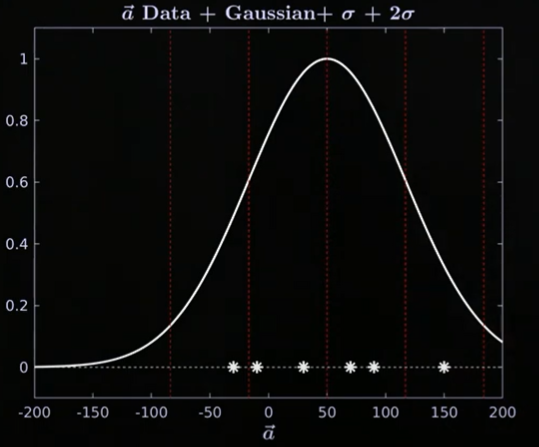
\includegraphics[scale=0.40]{./figures/vecAstd}
        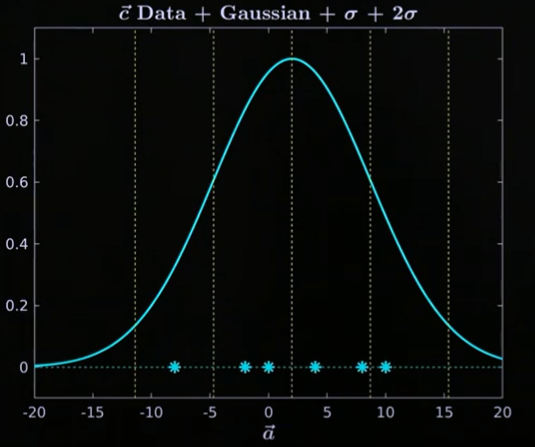
\includegraphics[scale=0.40]{./figures/vecCstd}
\end{figure}
\pagebreak


Thus we can measure and plot each data point in $\vec a$ and  $\vec c$ in terms of their respective standard deviations like so:
 \begin{figure}[h]
        \centering
        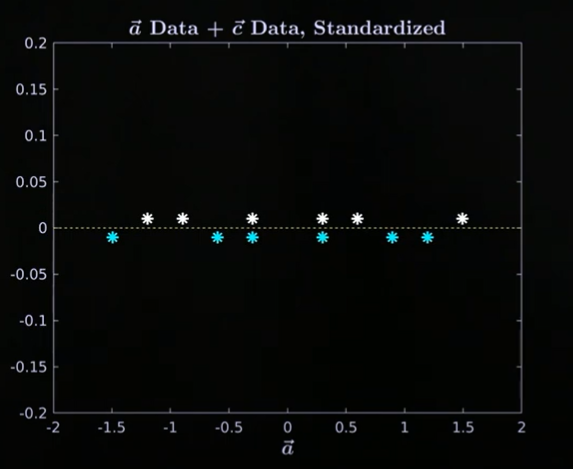
\includegraphics[scale=0.5]{./figures/stdData}
\end{figure}
\section*{Learning Outcomes}
Students should now be able to:
\begin{itemize}
        \item Determine whether data needs transposition
        \item Create Zero Mean Data
        \item Create Unit Variance Data
        \item Prepare data for analysis
\end{itemize}





\end{document}

